
\Needspace{8\baselineskip}\subsection{Les sections de câbles et les fusibles}

\subsubsection*{La chute de tension et la section minimale}

Je cherche, pour chaque liaison, la plus petite section de cuivre qui garde la chute de tension sous une limite, puis je prends la section normalisée immédiatement supérieure.

\naturecalc{théorie (formule démontrée, valeurs de fiches techniques et hypothèses ; rien de mesuré)}
\begin{demonstration}[section minimale d'un câble]
\resultat{S \geq \dfrac{2\,\rho\, L\, I}{\varepsilon\, U}}
Je note $\rho$ la résistivité du cuivre, en $\unit{\ohm\,mm^2/m}$, $L$ la longueur de la liaison, en mètres, $S$ la section, en mm$^2$, $I$ le courant, en ampères, $U$ la tension de la ligne, en volts, et $\varepsilon$ la chute de tension relative admise (sans unité). La résistance d'un conducteur de longueur $\ell$ et de section $S$ vaut :
\begin{align*}
R &= \rho\,\frac{\ell}{S}
\end{align*}
Le courant fait l'aller et le retour : pour une liaison de longueur $L$, la longueur de conducteur est $\ell = 2L$ :
\begin{align*}
R &= \frac{2\,\rho\, L}{S}
\end{align*}
La chute de tension se calcule par la loi d'Ohm :
\begin{align*}
\Delta U &= R\, I\\
\Delta U &= \frac{2\,\rho\, L\, I}{S}
\end{align*}
J'impose $\Delta U \leq \varepsilon\, U$ :
\begin{align*}
\frac{2\,\rho\, L\, I}{S} &\leq \varepsilon\, U\\
S &\geq \frac{2\,\rho\, L\, I}{\varepsilon\, U}
\end{align*}
La résistivité du cuivre augmente avec la température $T$ (en °C), avec le coefficient $\alpha_{Cu} = \qty{0,00393}{/\celsius}$ :
\begin{align*}
\rho(T) &= \rho_{20}\left[1 + \alpha_{Cu}\,(T - \qty{20}{\celsius})\right]
\end{align*}
\end{demonstration}

\naturecalc{théorie (formule démontrée, valeurs de fiches techniques et hypothèses ; rien de mesuré)}
\begin{demonstration}[résistivité du cuivre à 60 °C]
\resultat{\rho = \qty{0,0199}{\ohm.mm^2/m}}
Les câbles sont au soleil ou dans le boîtier chaud : je prends $T = \qty{60}{\celsius}$, et $\rho_{20} = \qty{0,0172}{\ohm.mm^2/m}$ :
\begin{align*}
\rho &= \qty{0,0172}{\ohm.mm^2/m} \times \left[1 + \qty{0,00393}{/\celsius} \times (\qty{60}{\celsius} - \qty{20}{\celsius})\right]\\
\rho &= \qty{0,0172}{\ohm.mm^2/m} \times 1{,}1572\\
\rho &\approx \qty{0,0199}{\ohm.mm^2/m}
\end{align*}
\end{demonstration}

\naturecalc{théorie (formule démontrée, valeurs de fiches techniques et hypothèses ; rien de mesuré)}
\begin{demonstration}[section du câble panneau vers régulateur]
\resultat{S \geq \qty{2,97}{mm^2}\ \Rightarrow\ S = \qty{4}{mm^2}}
Avec $L = \qty{5}{m}$, $I = \qty{6,83}{A}$ et $U = \qty{15,26}{V}$ (point de puissance maximale à \qty{54}{\celsius}), et $\varepsilon = 3\,\%$ :
\begin{align*}
S &\geq \frac{2 \times \qty{0,0199}{\ohm.mm^2/m} \times \qty{5}{m} \times \qty{6,83}{A}}{0{,}03 \times \qty{15,26}{V}}\\
S &\geq \frac{\qty{1,359}{\ohm.mm^2.A}}{\qty{0,458}{V}}\\
S &\geq \qty{2,97}{mm^2}
\end{align*}
Je choisis \qty{4}{mm^2} (câble solaire), la section normalisée immédiatement supérieure. La chute réelle vaut alors :
\begin{align*}
\Delta U &= \frac{2 \times \qty{0,0199}{\ohm.mm^2/m} \times \qty{5}{m} \times \qty{6,83}{A}}{\qty{4}{mm^2}}\\
\Delta U &\approx \qty{0,34}{V} \quad (2{,}2\,\%)
\end{align*}
\end{demonstration}

Les autres liaisons se calculent de la même façon. Le tableau donne, pour chacune, la longueur, le courant, la tension, la chute relative admise, la section minimale, la section retenue et la chute réelle.

\begin{table}[H]
\centering
\small
\begin{tabular}{|l|c|c|c|c|c|c|c|}
\hline
\textbf{Liaison} & \textbf{$L$ (m)} & \textbf{$I$ (A)} & \textbf{$U$ (V)} & \textbf{$\varepsilon$} & \textbf{$S_{\min}$ (mm$^2$)} & \textbf{$S$ (mm$^2$)} & \textbf{$\Delta U$ réel} \\
\hline
Panneau vers MPPT\ix{19} & 5,0 & 6,83 & 15,3 & 3\,\% & 2,97 & 4 & 2,2\,\% \\
\hline
MPPT\ix{19} vers INA260\ix{22} vers bus & 0,5 & 8,91 & 12,8 & 1\,\% & 1,38 & 4 & 0,35\,\% \\
\hline
Bus vers B1 (6 Ah) & 0,3 & 2,32 & 12,8 & 0,5\,\% & 0,43 & 2,5 & 0,09\,\% \\
\hline
Bus vers B2 (17 Ah) & 0,3 & 6,58 & 12,8 & 0,5\,\% & 1,23 & 2,5 & 0,25\,\% \\
\hline
Sortie LOAD vers bornier & 0,5 & 2,70 & 12,8 & 1\,\% & 0,42 & 1,5 & 0,28\,\% \\
\hline
Bornier vers circulation & 3,0 & 1,48 & 12,8 & 3\,\% & 0,46 & 1,5 & 0,92\,\% \\
\hline
Bornier vers doseuse & 1,0 & 0,30 & 12,8 & 3\,\% & 0,03 & 0,5 & 0,19\,\% \\
\hline
UBEC\ix{17} vers Pi (\qty{5}{V}) & 0,3 & 1,00 & 5,0 & 2\,\% & 0,12 & 0,5 & 0,48\,\% \\
\hline
\end{tabular}
\caption{Sections de câbles : $\rho = \qty{0,0199}{\ohm.mm^2/m}$ à \qty{60}{\celsius}, chute admise $\varepsilon$ propre à chaque liaison (\qty{3}{\percent} côté panneau et pompes, \qty{1}{\percent} côté batterie, \qty{0,5}{\percent} entre batteries, \qty{2}{\percent} sur le \qty{5}{V}).}
\end{table}

La chute totale du panneau aux batteries vaut environ $2{,}2 + 0{,}35 = \qty{2,6}{\percent}$ au courant maximal, et nettement moins en moyenne sur la journée : le facteur $k_{câbles} = 0{,}98$ est cohérent. Sur le \qty{5}{V} du Pi, une chute supérieure à \qty{0,25}{V} provoque des alertes de sous-tension : le câble court de \qty{0,5}{mm^2} est indispensable (il faut éviter un câble USB fin et long).

\subsubsection*{Les fusibles}

\naturecalc{théorie (formule démontrée, valeurs de fiches techniques et hypothèses ; rien de mesuré)}
\begin{demonstration}[règle de choix d'un fusible]
\resultat{1{,}25\, I_b \leq I_n \leq I_z}
Je note $I_b$ le courant normal maximal dans la ligne, en ampères, $I_n$ le calibre du fusible, en ampères, et $I_z$ le courant admissible du câble protégé, en ampères. Le fusible doit laisser passer le courant normal maximal sans fondre ni vieillir : je prends une marge de 25\,\%.
\begin{align*}
I_n &\geq 1{,}25\, I_b
\end{align*}
Il doit aussi fondre avant que le câble chauffe dangereusement, donc rester sous le courant admissible du câble :
\begin{align*}
1{,}25\, I_b &\leq I_n \leq I_z
\end{align*}
On prend le calibre normalisé immédiatement supérieur à $1{,}25\, I_b$ (valeurs courantes : 1, 2, 3, 4, 5, 7,5, 10, 15, 20 A).
\end{demonstration}

\naturecalc{théorie (formule démontrée, valeurs de fiches techniques et hypothèses ; rien de mesuré)}
\begin{demonstration}[calibres des fusibles]
\resultat{F_{PV} = \qty{10}{A},\ F_{B1} = \qty{5}{A},\ F_{B2} = \qty{15}{A},\ F_2 = \qty{4}{A},\ F_3 = \qty{2}{A}}
$F_{PV}$ (panneau). Le courant maximal est le courant de court-circuit, augmenté à chaud :
\begin{align*}
1{,}25 \times \qty{7,3}{A} &= \qty{9,1}{A}\ \Rightarrow\ I_n = \qty{10}{A}
\end{align*}
C'est aussi le calibre maximal autorisé par l'étiquette du panneau.

$F_{B1}$ (batterie de \qty{6}{Ah}). Courant normal en charge \qty{2,32}{A} :
\begin{align*}
1{,}25 \times \qty{2,32}{A} &= \qty{2,9}{A}\ \Rightarrow\ I_n = \qty{5}{A}\ \text{(conservé)}
\end{align*}
Si le BMS de B2 coupe, les \qty{8,9}{A} de charge passeraient dans B1 : le fusible de \qty{5}{A} fond et protège la petite batterie.

$F_{B2}$ (batterie de \qty{17}{Ah}). Normalement \qty{6,58}{A}, mais jusqu'à \qty{8,9}{A} si B1 est déconnectée :
\begin{align*}
1{,}25 \times \qty{8,9}{A} &= \qty{11,1}{A}\ \Rightarrow\ I_n = \qty{15}{A}\ \text{(conservé)}
\end{align*}
En plomb AGM (\qty{9,5}{A} de charge), $1{,}25 \times \qty{9,5}{A} = \qty{11,9}{A}$ conduit au même calibre de \qty{15}{A}.

$F_2$ (sortie LOAD, toutes les charges). Le courant maximal est celui de la circulation, des trois doseuses ensemble (cas extrême) et de l'électronique :
\begin{align*}
I_b &= \qty{1,48}{A} + 3 \times \qty{0,30}{A} + \qty{0,30}{A}\\
I_b &= \qty{2,68}{A}\\
1{,}25 \times \qty{2,68}{A} &= \qty{3,4}{A}\ \Rightarrow\ I_n = \qty{4}{A}
\end{align*}
La version 1 prévoyait \qty{7,5}{A} avec la pompe d'appoint ; sans elle, \qty{4}{A} protège mieux.

\textbf{Limite de ce calcul.} Il part des courants permanents. Au démarrage, un moteur à courant continu peut absorber brièvement un courant plus grand que son courant nominal, et la fiche de la pompe ne donne pas cette valeur. Je ne peux donc pas valider définitivement le calibre de \qty{4}{A} : je mesurerai le pic de démarrage de la circulation et des doseuses avec l'INA260\ix{22} ou une pince ampèremétrique. Si le pic dure plus de quelques dizaines de millisecondes au-dessus de \qty{4}{A}, je prendrai un fusible temporisé, et je vérifierai dans la fiche de la carte MOSFET\ix{15} qu'elle supporte ce pic.

$F_3$ (entrée de l'UBEC\ix{17}). Le courant d'entrée maximal si l'UBEC\ix{17} fournit ses \qty{3}{A} nominaux se déduit du rendement : $P_{entrée} = P_{sortie}/\eta$, donc $I_{entrée} = P_{sortie}/(\eta\, U_B)$ :
\begin{align*}
I_{entrée,max} &= \frac{\qty{5}{V} \times \qty{3}{A}}{0{,}83 \times \qty{12,8}{V}}\\
I_{entrée,max} &\approx \qty{1,41}{A}\\
1{,}25 \times \qty{1,41}{A} &= \qty{1,8}{A}\ \Rightarrow\ I_n = \qty{2}{A}
\end{align*}
\end{demonstration}

Le tableau suivant donne le calibre retenu pour chaque fusible de la tour.

\begin{table}[H]
\centering
\small
\begin{tabular}{|l|l|c|c|c|}
\hline
\textbf{Fusible} & \textbf{Emplacement} & \textbf{$I_b$ (A)} & \textbf{Calibre v1} & \textbf{Calibre v2} \\
\hline
$F_{PV}$ & panneau, borne $+$ & 7,3 & \qty{10}{A} & \qty{10}{A} \\
\hline
$F_{B1}$ & batterie \qty{6}{Ah}, borne $+$ & 2,32 & \qty{5}{A} & \qty{5}{A} \\
\hline
$F_{B2}$ & batterie \qty{17}{Ah}, borne $+$ & 6,58 (8,9) & \qty{15}{A} & \qty{15}{A} \\
\hline
$F_2$ & sortie LOAD du MPPT\ix{19} & 2,68 & \qty{7,5}{A} & \qty{4}{A} \\
\hline
$F_3$ & entrée de l'UBEC\ix{17} & 0,30 (1,41) & absent & \qty{2}{A} \\
\hline
\end{tabular}
\caption{Calibres des fusibles de la tour.}
\end{table}

\textbf{Autres vérifications.} L'INA260\ix{22} supporte \qty{15}{A} en continu : avec $F_{B2} = \qty{15}{A}$ en amont et \qty{8,9}{A} au maximum en fonctionnement, il est protégé (le régulateur peut débiter \qty{20}{A}, mais le panneau ne peut pas dépasser \qty{7,3}{A} de courant de court-circuit, soit moins de \qty{10}{A} côté batterie). La tension maximale du panneau, le matin frais à $T_c = \qty{20}{\celsius}$, vaut $22{,}0 - 0{,}080 \times (20 - 25) = \qty{22,4}{V}$ : elle est très inférieure aux \qty{70}{V} d'entrée admis par la fiche du régulateur. Chaque canal de la carte 6318 supporte \qty{3,6}{A} en pointe : la circulation (\qty{0,74}{A} par canal) et les doseuses (\qty{0,30}{A}) sont loin de cette limite.

\begin{aretenir}
Câbles : \qty{4}{mm^2} du panneau vers le régulateur (chute \qty{2,2}{\percent}) et du régulateur vers le bus, \qty{2,5}{mm^2} vers chaque batterie, \qty{1,5}{mm^2} pour la sortie LOAD et la pompe de circulation, \qty{0,5}{mm^2} pour les doseuses et le \qty{5}{V} du Pi. Fusibles : $F_{PV} = \qty{10}{A}$, $F_{B1} = \qty{5}{A}$, $F_{B2} = \qty{15}{A}$ (inchangés), $F_2 = \qty{4}{A}$ (au lieu de \qty{7,5}{A}), nouveau $F_3 = \qty{2}{A}$ en entrée de l'UBEC\ix{17}.
\end{aretenir}

\Needspace{8\baselineskip}\subsection{Le protocole de mesure}

Ce protocole permet de remplacer les hypothèses de cette étude par des valeurs mesurées. Il s'appuie sur trois fichiers : un modèle vide de relevé pour les mesures ponctuelles M1, M2, M4 et M5, un modèle vide pour l'enregistrement d'une journée (M3), et un script de traitement. Lancé sans argument, le script fonctionne sur des données d'\textbf{exemple} fictives, ce qui prouve qu'il marche.

\textbf{Matériel.} Il faut un multimètre avec calibre \qty{10}{A} continu, l'INA260\ix{22} déjà câblé (lecture par l'Arduino, relayée au Raspberry Pi), un testeur USB (courant \qty{5}{V}) si disponible, une éprouvette graduée de \qty{100}{mL} et un chronomètre, un thermomètre infrarouge (facultatif) et les fiches de relevé ci-dessous.

\begin{attention}
Ne jamais brancher le multimètre en ampèremètre en parallèle sur la batterie : c'est un court-circuit. Il faut ouvrir le circuit, brancher le multimètre en série, puis refermer. Il faut aussi retirer le fusible concerné pendant les manipulations de câbles.
\end{attention}

\subsubsection*{M1 : le courant de chaque pompe}

Je retire $F_2$, je débranche le fil $+$ de la pompe sur la carte 6318 et j'insère le multimètre (calibre \qty{10}{A}) en série. Je remets $F_2$ et je commande la pompe depuis le Pi (par exemple \texttt{D 0 60000} pour la circulation, \texttt{D 1 10000} pour l'engrais A). Je relève le courant après \qty{5}{s} de marche (régime établi) et la tension aux bornes de la pompe. Je recommence pour chaque pompe ; pour les doseuses, le tuyau doit être en charge (plongé dans le liquide). Je fais aussi une mesure de la circulation sous \qty{14,4}{V} (batterie en fin de charge), car un moteur à courant continu consomme plus quand la tension monte.

La fiche de relevé M1, ci-dessous, sert à noter les mesures de cet essai.

\begin{table}[H]
\centering
\small
\begin{tabular}{|p{4.2cm}|p{2.2cm}|p{2.2cm}|p{2.2cm}|p{2.8cm}|}
\hline
\textbf{Pompe} & \textbf{$U$ mesurée (V)} & \textbf{$I$ mesuré (A)} & \textbf{$P = UI$ (W)} & \textbf{Théorie} \\
\hline
Circulation (canaux 0 + 1) & & & & \qty{1,48}{A}, \qty{19}{W} \\[6pt]
\hline
Doseuse engrais A & & & & \qty{0,30}{A} \\[6pt]
\hline
Doseuse engrais B & & & & \qty{0,30}{A} \\[6pt]
\hline
Doseuse pH$-$ & & & & \qty{0,30}{A} \\[6pt]
\hline
\end{tabular}
\caption{Fiche de relevé M1.}
\end{table}

\subsubsection*{M2 : la consommation au repos et le rendement de l'UBEC}

La nuit (pas de charge), toutes les pompes arrêtées et le Pi en fonctionnement normal, je relève le courant de la batterie donné par l'INA260\ix{22} pendant \qty{10}{min} (une valeur par minute) et j'en fais la moyenne. Je contrôle une valeur au multimètre en série sur la sortie LOAD. Si un testeur USB est disponible, je mesure le courant \qty{5}{V} du Pi et je calcule le rendement $\eta = (U_5\, I_5)/(U_{12}\, I_{12})$.

La fiche de relevé M2, ci-dessous, sert à noter les mesures de cet essai.

\begin{table}[H]
\centering
\small
\begin{tabular}{|p{5cm}|p{3cm}|p{3cm}|p{3cm}|}
\hline
\textbf{Grandeur} & \textbf{Mesure} & \textbf{Unité} & \textbf{Théorie} \\
\hline
Courant de repos \qty{12}{V} (INA260\ix{22}, moyenne) & & A & 0,314 \\[6pt]
\hline
Courant de repos \qty{12}{V} (multimètre) & & A & 0,314 \\[6pt]
\hline
Tension de sortie UBEC\ix{17} & & V & 5,0 \\[6pt]
\hline
Courant \qty{5}{V} (testeur USB) & & A & 0,635 \\[6pt]
\hline
Rendement UBEC\ix{17} calculé & & sans unité & 0,83 \\[6pt]
\hline
\end{tabular}
\caption{Fiche de relevé M2.}
\end{table}

\subsubsection*{M3 : la production et le bilan sur une journée}

Je choisis une journée représentative et je note la météo (ensoleillé, nuageux, pluie). J'enregistre toutes les \qty{5}{min}, de 0 h à 24 h, la tension et le courant de la batterie donnés par l'INA260\ix{22} (le Raspberry Pi peut les écrire directement dans le fichier ; le courant est positif en charge). De 6 h à 18 h, je relève toutes les \qty{30}{min} la tension et le courant du panneau (afficheur du régulateur ou multimètre), et je mets 0 la nuit : toutes les lignes doivent être remplies. Je note l'état de la pompe de circulation (1 marche, 0 arrêt). Je lance enfin le script de traitement sur le fichier de la journée et sur celui des mesures ponctuelles.

La fiche de relevé M3, ci-dessous, sert à noter les mesures de cet essai.

\begin{table}[H]
\centering
\small
\begin{tabular}{|p{1.4cm}|p{2.0cm}|p{2.0cm}|p{2.0cm}|p{2.0cm}|p{1.4cm}|p{2.0cm}|}
\hline
\textbf{Heure} & \textbf{$U_{bat}$ (V)} & \textbf{$I_{bat}$ (A)} & \textbf{$I_{PV}$ (A)} & \textbf{$U_{PV}$ (V)} & \textbf{Pompe} & \textbf{Remarque} \\
\hline
06:00 & & & & & & \\
\hline
08:00 & & & & & & \\
\hline
10:00 & & & & & & \\
\hline
12:00 & & & & & & \\
\hline
14:00 & & & & & & \\
\hline
16:00 & & & & & & \\
\hline
18:00 & & & & & & \\
\hline
\end{tabular}
\caption{Fiche de relevé M3 (extrait : le fichier complet contient une ligne toutes les \qty{5}{min}).}
\end{table}

\subsubsection*{M4 : la tension des batteries et leur identification}

Je lis et je note l'étiquette de chaque batterie (technologie, capacité, tension de charge, courant maximal). Avant de les relier, je mesure la tension à vide de chaque batterie au multimètre. Je mesure la tension du bus au repos avant l'aube (fin de nuit), puis à midi en charge, et pendant une marche de la pompe. Je compare chaque valeur à celle de l'INA260\ix{22} : l'écart attendu est inférieur à \qty{0,05}{V}.

\begin{table}[H]
\centering
\small
\begin{tabular}{|p{5.2cm}|p{2.6cm}|p{2.6cm}|p{3.6cm}|}
\hline
\textbf{Situation} & \textbf{Multimètre (V)} & \textbf{INA260\ix{22} (V)} & \textbf{Repère LiFePO4} \\
\hline
Technologie B1 / B2 (étiquette) & \multicolumn{2}{l|}{} & identiques ? \\[6pt]
\hline
B1 seule, à vide & & & 13,0 à 13,4 \\[6pt]
\hline
B2 seule, à vide & & & 13,0 à 13,4 \\[6pt]
\hline
Bus, fin de nuit (repos) & & & $\geq 13{,}0$ \\[6pt]
\hline
Bus, midi en charge & & & 13,8 à 14,6 \\[6pt]
\hline
Bus, pompe en marche & & & \\[6pt]
\hline
\end{tabular}
\caption{Fiche de relevé M4.}
\end{table}

\subsubsection*{M5 : le débit des pompes doseuses}

Je plonge le tuyau d'aspiration dans de l'eau et je place la sortie dans l'éprouvette. Je commande la pompe \qty{30}{s} (\texttt{D 1 30000}) et je lis le volume. Le débit vaut $Q = V/t$ ; je refais l'essai 3 fois et je fais la moyenne.

La fiche de relevé M5, ci-dessous, sert à noter les mesures de cet essai.

\begin{table}[H]
\centering
\small
\begin{tabular}{|p{3.6cm}|p{2.4cm}|p{2.4cm}|p{2.4cm}|p{3cm}|}
\hline
\textbf{Pompe} & \textbf{Essai 1 (mL)} & \textbf{Essai 2 (mL)} & \textbf{Essai 3 (mL)} & \textbf{$Q$ moyen (mL/min)} \\
\hline
Engrais A & & & & \\[6pt]
\hline
Engrais B & & & & \\[6pt]
\hline
pH$-$ & & & & \\[6pt]
\hline
\end{tabular}
\caption{Fiche de relevé M5.}
\end{table}

\subsubsection*{Le traitement : l'énergie par la méthode des trapèzes}

\naturecalc{théorie (formule démontrée, valeurs de fiches techniques et hypothèses ; rien de mesuré)}
\begin{demonstration}[méthode des trapèzes]
\resultat{E \approx \sum_{k=0}^{N-1} (t_{k+1} - t_k)\,\dfrac{p_k + p_{k+1}}{2}}
Je note $p(t) = u(t)\, i(t)$ la puissance, en watts, $t_k$ les instants de relevé, en heures, et $p_k = p(t_k)$. L'énergie est l'intégrale de la puissance, mais on ne connaît $p$ qu'aux instants de relevé $t_0, t_1, \dots, t_N$. Entre deux relevés, je remplace $p$ par le segment de droite qui joint $(t_k, p_k)$ et $(t_{k+1}, p_{k+1})$ :
\begin{align*}
p(t) &\approx p_k + \frac{p_{k+1} - p_k}{t_{k+1} - t_k}\,(t - t_k)
\end{align*}
J'intègre cette droite sur $[t_k, t_{k+1}]$, en posant $h = t_{k+1} - t_k$ et $\tau = t - t_k$ :
\begin{align*}
\int_{t_k}^{t_{k+1}} p(t)\,\mathrm{d}t &\approx \int_{0}^{h}\left(p_k + \frac{p_{k+1} - p_k}{h}\,\tau\right)\mathrm{d}\tau\\
&= p_k\, h + \frac{p_{k+1} - p_k}{h}\cdot\frac{h^2}{2}\\
&= h\,\frac{p_k + p_{k+1}}{2}
\end{align*}
C'est l'aire d'un trapèze de bases $p_k$ et $p_{k+1}$ et de hauteur $h$. J'additionne tous les intervalles :
\begin{align*}
E &\approx \sum_{k=0}^{N-1} (t_{k+1} - t_k)\,\frac{p_k + p_{k+1}}{2}
\end{align*}
Avec $t$ en heures et $p$ en watts, $E$ est en wattheures.
\end{demonstration}

Le script calcule ainsi l'énergie produite par le panneau $E_{PV}$ et l'énergie nette entrée dans la batterie $E_{net}$. Il en déduit la consommation journalière par le bilan :
\begin{align*}
E_{cons} &= k_{MPPT}\, E_{PV} - E_{net}
\end{align*}
c'est-à-dire ce que le régulateur fournit, moins ce qui reste stocké dans la batterie. Il compare $E_{PV}$ à \qty{304,5}{Wh/j}, $E_{cons}$ à \qty{226,7}{Wh/j} et chaque mesure ponctuelle à sa valeur théorique.

\textbf{Résultat sur les données d'exemple.} Ces données sont \emph{fictives} (une journée nuageuse simulée) ; elles servent uniquement à prouver que le script fonctionne.

Le tableau suivant reproduit la sortie du script sur les données d'exemple.

\begin{table}[H]
\centering
\small
\begin{tabular}{|l|r|r|r|}
\hline
\textbf{Grandeur (exemple)} & \textbf{Calcul} & \textbf{Théorie} & \textbf{Écart} \\
\hline
Énergie produite par le panneau & \qty{301,4}{Wh/j} & \qty{304,5}{Wh/j} & $-$1,0\,\% \\
\hline
Énergie nette entrée dans la batterie & \qty{61,1}{Wh/j} & & \\
\hline
Consommation déduite du bilan & \qty{225,3}{Wh/j} & \qty{226,7}{Wh/j} & $-$0,6\,\% \\
\hline
Courant de la pompe de circulation & \qty{1,52}{A} & \qty{1,48}{A} & $+$2,4\,\% \\
\hline
Courant de repos \qty{12}{V} & \qty{0,33}{A} & \qty{0,314}{A} & $+$5,1\,\% \\
\hline
\end{tabular}
\caption{Sortie du script sur les données d'exemple (fictives).}
\end{table}

La figure suivante est le tracé que produit le même script sur ces données d'exemple.

\begin{figure}[H]
\centering
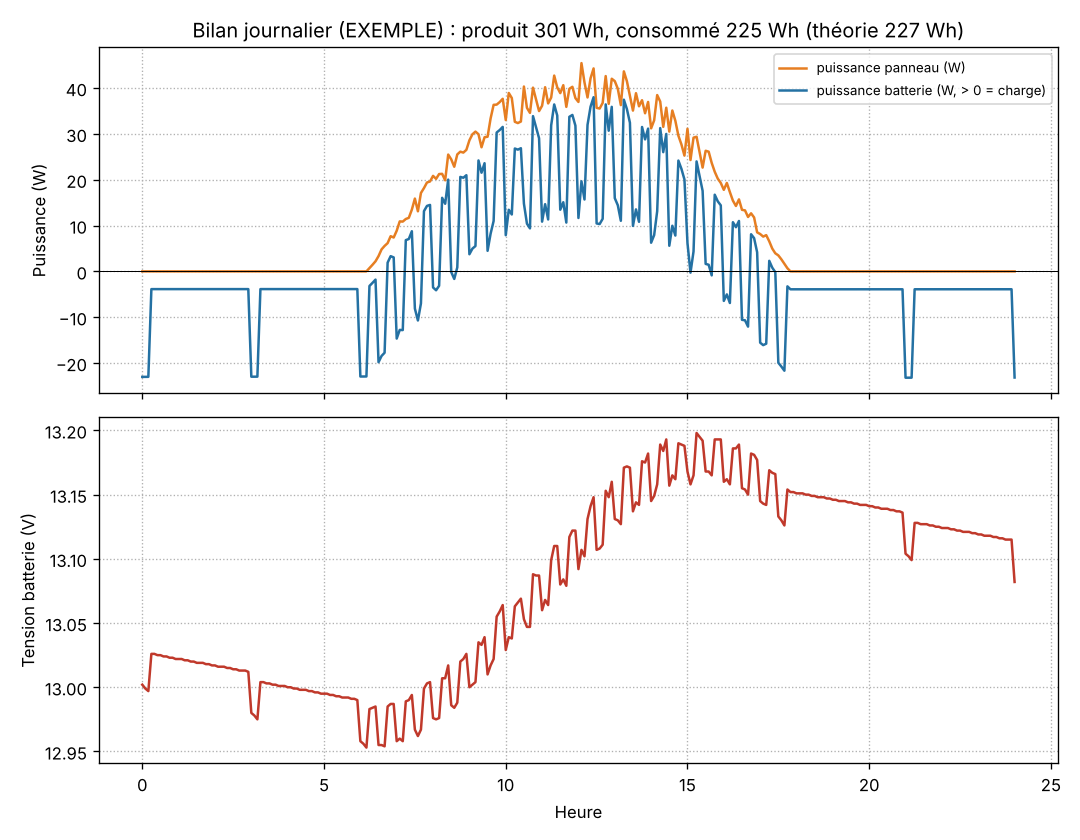
\includegraphics[width=0.9\textwidth]{img/elec/exemple_bilan_journee.png}
\caption{Sortie du script sur les données d'exemple : puissances du panneau et de la batterie, tension de la batterie.}
\end{figure}

\begin{figure}[H]
\centering
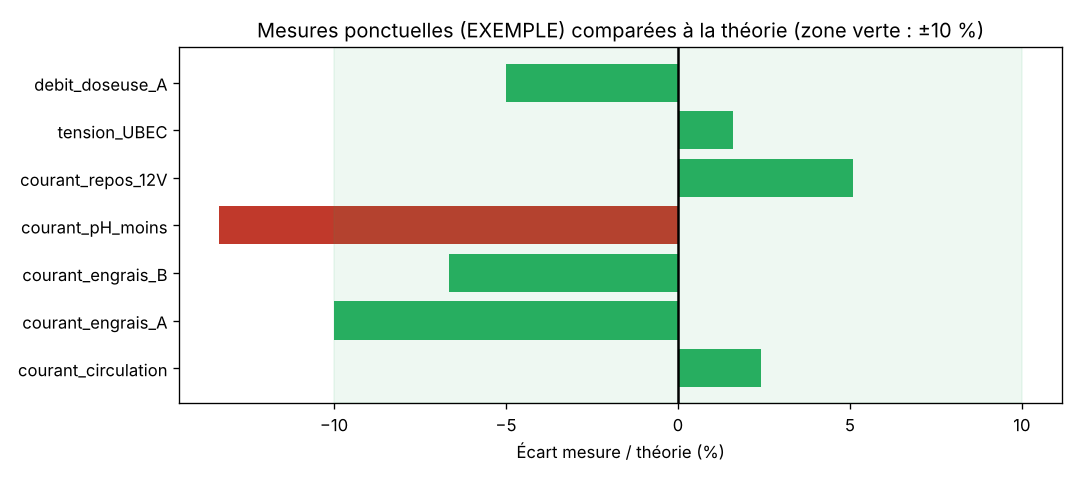
\includegraphics[width=0.85\textwidth]{img/elec/exemple_ecarts.png}
\caption{Sortie du script sur les données d'exemple : écart entre les mesures ponctuelles et la théorie.}
\end{figure}

\textbf{Exploitation.} Si un écart dépasse \qty{10}{\percent}, je remplace l'hypothèse correspondante par la valeur mesurée dans le calcul, je relance le calcul et je mets à jour le bilan de la partie 5.3. Les chiffres de cette partie sont calculés : aucune mesure réelle n'est encore faite.

\begin{aretenir}
Cinq séries de mesures : le courant de chaque pompe (M1), la consommation au repos et le rendement de l'UBEC\ix{17} (M2), le bilan d'une journée enregistré par l'INA260\ix{22} toutes les \qty{5}{min} (M3), les tensions et l'identification des batteries (M4), le débit des doseuses (M5). Le script intègre les puissances par la méthode des trapèzes, déduit la consommation réelle et la compare à la théorie ; il a été vérifié sur des données d'exemple.
\end{aretenir}

\Needspace{8\baselineskip}\subsection{Les hypothèses de l'étude}

Chaque hypothèse est à confirmer, par les mesures M1 à M5 du protocole ou par la lecture des étiquettes et des notices.

\textbf{Données reprises de la version 1.} Le TE1250 a une puissance crête de \qty{120}{Wc}, une puissance minimale de \qty{117,5}{W}, $V_{mp} = \qty{17,6}{V}$, $I_{mp} = \qty{6,8}{A}$, $I_{sc} = \qty{7,3}{A}$, $V_{oc} = \qty{22,0}{V}$ et un fusible série maximal de \qty{10}{A}. L'irradiation du pire mois n'est plus reprise de la version 1 : elle vient de Solargis (juin, $H = \qty{3,607}{kWh/m^2/j}$, partie 5.4). Le rendement du convertisseur \qty{12}{V} vers \qty{5}{V} est de $0{,}83$.

\textbf{Panneau.} Les coefficients de température du TE1250 sont pris égaux à ceux du SLP055 (même technologie à 36 cellules) : $V_{oc}$ de $-\qty{80}{mV/\celsius}$, $I_{sc}$ de $+\qty{0,065}{\percent/\celsius}$, $P_{\max}$ de $-\qty{0,5}{\percent/\celsius}$, NOCT de \qty{47}{\celsius}. Le TE1250 a 36 cellules en série (cohérent avec $V_{oc} = \qty{22}{V}$). Le calcul se fait directement sur le panneau entier, sans modèle de cellule. La température de l'air en milieu de journée du pire mois est de \qty{27}{\celsius}, et l'éclairement de calcul de la température de cellule de \qty{800}{W/m^2}, d'où $T_c = \qty{54}{\celsius}$. Les facteurs de pertes sont 0,95 (salissures, sel et orientation), 0,95 (régulateur MPPT\ix{19}), 0,98 (câbles) et 0,95 (LiFePO4) ou 0,85 (AGM) pour la batterie, appliqué à toute l'énergie (prudent). Un jour très couvert apporte \qty{1,2}{kWh/m^2/j}.

\textbf{Consommation.} Le Raspberry Pi 3 B sans écran, en charge faible, consomme \qty{450}{mA} en moyenne à \qty{5}{V} (plage typique de \qty{260}{mA} à \qty{500}{mA} au repos, plus en charge). Le dongle Wi-Fi USB à antenne externe consomme \qty{120}{mA} en moyenne (émission intermittente). L'Arduino Uno R3 consomme \qty{50}{mA}, les capteurs leurs courants de fiche typiques, et la sonde EC n'est alimentée que 2 secondes par minute environ. La pompe de circulation consomme \qty{19}{W} (\qty{1,48}{A} à \qty{12,8}{V}) avec un planning de \qty{6,75}{h/j}. Le MOSFET\ix{15} de la carte 6318 a $R_{DS(on)} = \qty{70}{m\ohm}$ par canal. Les pompes doseuses consomment \qty{0,30}{A} sous \qty{12}{V} et débitent \qty{80}{mL/min} en charge (la fiche annonce jusqu'à \qty{100}{mL/min} à vide). Pour le dosage, je suppose une baisse d'EC de \qty{0,05}{mS/cm} par jour dans \qty{152}{L}, une sensibilité de la solution mère de \qty{0,56}{mS/cm} pour \qty{1}{mL/L} de A et de B, et \qty{6}{mL/j} de pH$-$ ; l'énergie retenue est un majorant de 10 commandes de \qty{30}{s} par pompe et par jour (\qty{0,96}{Wh/j}). L'autoconsommation du régulateur est de \qty{15}{mA} à \qty{12,8}{V}. La nuit de calcul dure 14 h (de 17 h à 7 h), avec 7 marches de \qty{15}{min} de la circulation.

\textbf{Batteries.} Mes batteries sont au plomb (Yuasa NP17-12I au plomb étanche, Steco de type AGM à confirmer sur son étiquette), alors que le cahier des charges de départ parlait de LiFePO4 : les deux cas sont donc calculés, et le plomb AGM est retenu pour les conclusions. En LiFePO4 : \qty{12,8}{V}, DoD\ix{27} 80\,\%, rendement 0,95, charge admise $0{,}5\,C$, absorption de \qty{14,2}{V} à \qty{14,6}{V}. En AGM : \qty{12,0}{V}, DoD\ix{27} 50\,\%, rendement 0,85, charge conseillée $0{,}25\,C$, absorption de \qty{14,4}{V} à \qty{14,7}{V}. La résistance interne de la batterie de \qty{6}{Ah} est supposée de \qty{60}{m\ohm}, celle de la \qty{17}{Ah} se déduit par proportion inverse à la capacité (\qty{21}{m\ohm}). Le seuil de mode sobriété proposé est de \qty{12,9}{V} au repos (LiFePO4), à ajuster.

\textbf{Câbles et fusibles.} La résistivité du cuivre à \qty{60}{\celsius} est de \qty{0,0199}{\ohm.mm^2/m}. Les longueurs sont de \qty{5}{m} du panneau au régulateur, \qty{0,5}{m} du régulateur au bus, \qty{0,3}{m} du bus à chaque batterie, \qty{0,5}{m} de la sortie LOAD au bornier, \qty{3}{m} du bornier à la pompe de circulation, \qty{1}{m} vers les doseuses et \qty{0,3}{m} de l'UBEC\ix{17} au Pi. Les chutes admises sont de \qty{3}{\percent} côté panneau et pompes, \qty{1}{\percent} côté batterie, \qty{0,5}{\percent} entre batteries et \qty{2}{\percent} sur le \qty{5}{V}. Le régulateur est à positif commun d'après sa notice : $PV-$, $BAT-$ et $LOAD-$ sont trois bornes séparées, qu'il ne faut jamais relier entre elles. Sa tension d'entrée maximale, \qty{70}{V} d'après la fiche, est très supérieure aux \qty{22,4}{V} du panneau à froid.

\Needspace{8\baselineskip}\subsection{La synthèse de l'étude électrique}

Le tableau suivant résume les résultats de l'étude électrique.

\begin{table}[H]
\centering
\small
\begin{tabular}{|l|c|c|}
\hline
\textbf{Résultat} & \textbf{Version 1} & \textbf{Version 2} \\
\hline
Consommation journalière & \qty{281}{Wh/j} & \qty{226,7}{Wh/j} \\
\hline
Production théorique (\qty{120}{Wc}) & \qty{504}{Wh/j} ($H = 4{,}2$) & \qty{432,8}{Wh/j} ($H = \num{3,607}$, juin) \\
\hline
Production disponible le pire mois & \qty{336}{Wh/j} & \qty{304,5}{Wh/j} (LiFePO4) / \qty{272,4}{Wh/j} (AGM) \\
\hline
Marge du panneau & $+20\,\%$ & $+34\,\%$ (LiFePO4) / $+20\,\%$ (AGM) \\
\hline
Énergie utilisable des batteries (\qty{23}{Ah}) & & \qty{235,5}{Wh} (LiFePO4) / \qty{138,0}{Wh} (AGM) \\
\hline
Part de la nuit dans l'énergie utilisable & & 38\,\% (LiFePO4) / 65\,\% (AGM) \\
\hline
Autonomie sans soleil & & \qty{1,0}{j} (LiFePO4) / \qty{0,6}{j} (AGM) \\
\hline
Fusibles & 10 / 5 / 15 / \qty{7,5}{A} & 10 / 5 / 15 / \qty{4}{A} + \qty{2}{A} (UBEC\ix{17}) \\
\hline
\end{tabular}
\caption{Synthèse de l'étude électrique.}
\end{table}

\begin{aretenir}
Le panneau TE1250 de \qty{120}{Wc} couvre le besoin du pire mois, juin (\qty{272}{Wh/j} pour \qty{227}{Wh/j} en plomb AGM, soit $+20\,\%$). Les batteries de \qty{23}{Ah} couvrent la nuit sans difficulté, mais seulement un à deux jours très couverts en LiFePO4 (un seul en AGM) : un mode sobriété basé sur la tension de la batterie est à programmer. Points à vérifier en priorité : la technologie réelle des deux batteries (étiquette de la Steco), le réglage du régulateur et le câblage séparé de ses trois bornes négatives, le courant de charge maximal réglable, puis les mesures M1 à M5.
\end{aretenir}
